% format the chapter/section details
\chapter{Results}
\label{chap:results}

% insert your text below the line
%-------------------------------------------
This chapter addresses the results from this study as they relate to each of the hypotheses in chapter \ref{chap:intro}. Additional results as they were made apparent in the data will be discussed thereafter.

\section{Hypothesis Driven Results}
\subsection{Environmental Spatial Variabilities}
Previous observational based efforts have found greater spatial variability in non-tornadic inflow environments compared to tornadic storm environments \citep{parker2014composite}. Given their dataset of rawinsonde launches, these variances were displayed through SRH and composite wind profiles (Fig. \ref{fig:parker_comp}). Using similar methodology, we can assess this dataset in a near and far-field perspective. First, an assessment of the number of profiles making up each spatial bin must be addressed (Fig. \ref{fig:space_nprofs}). Composite profiles can then be created showing near and far-field hodographs in tornadic and non-tornadic storms (Fig. \ref{fig:inflow_hodos}). In this work, the near-field will be used to describe the inflow environment up to 30 kilometers away in the x-direction. Far-field will consist of data beyond the 30 kilometer threshold. 

\begin{figure}[h!]
    \centering
    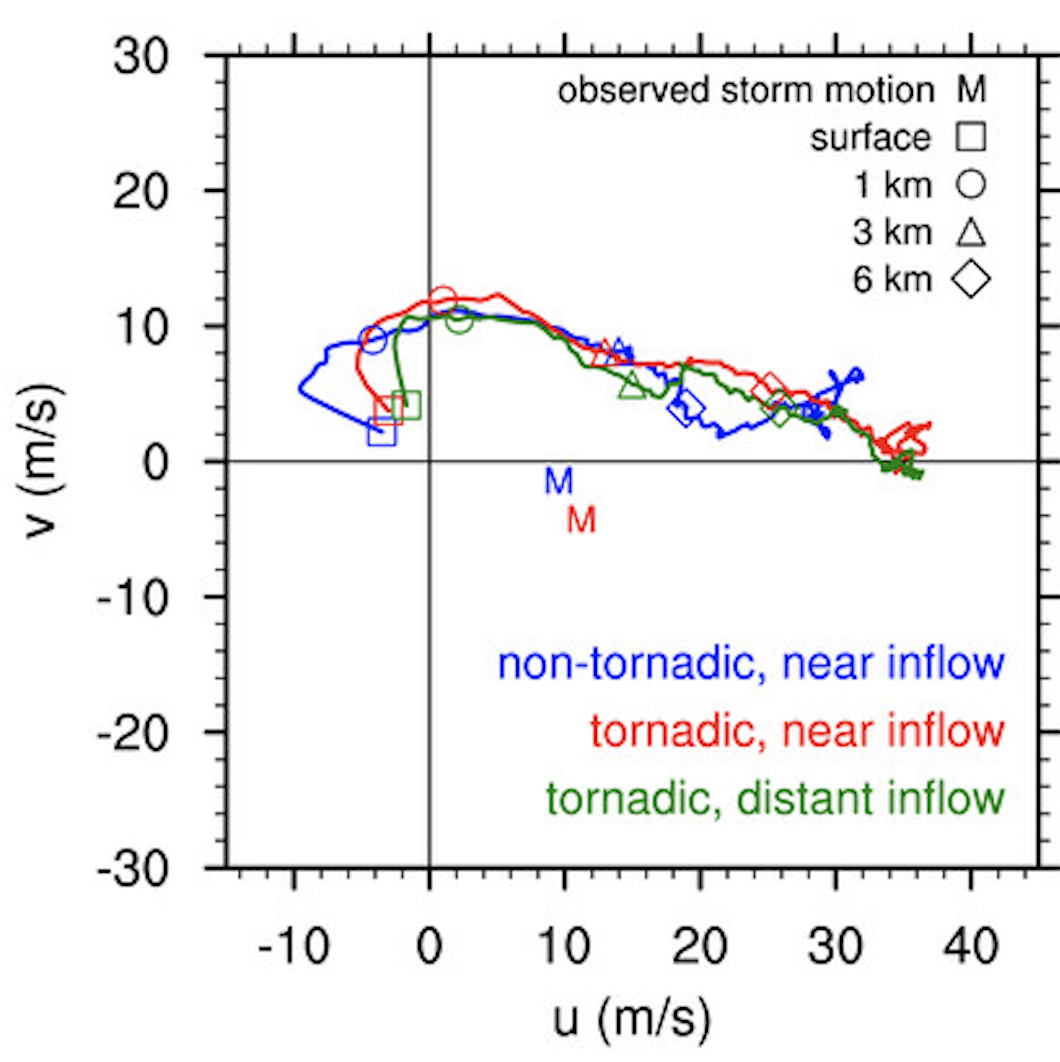
\includegraphics[width = 1\textwidth]{Figures/parker_composite.png}
    \caption{VORTEX-2 composite wind profiles, drawn from rawinsonde launches. From \cite{parker2014composite}; their figure 12.}
    \label{fig:parker_comp}
\end{figure}

\begin{figure}[h!]
    \centering
    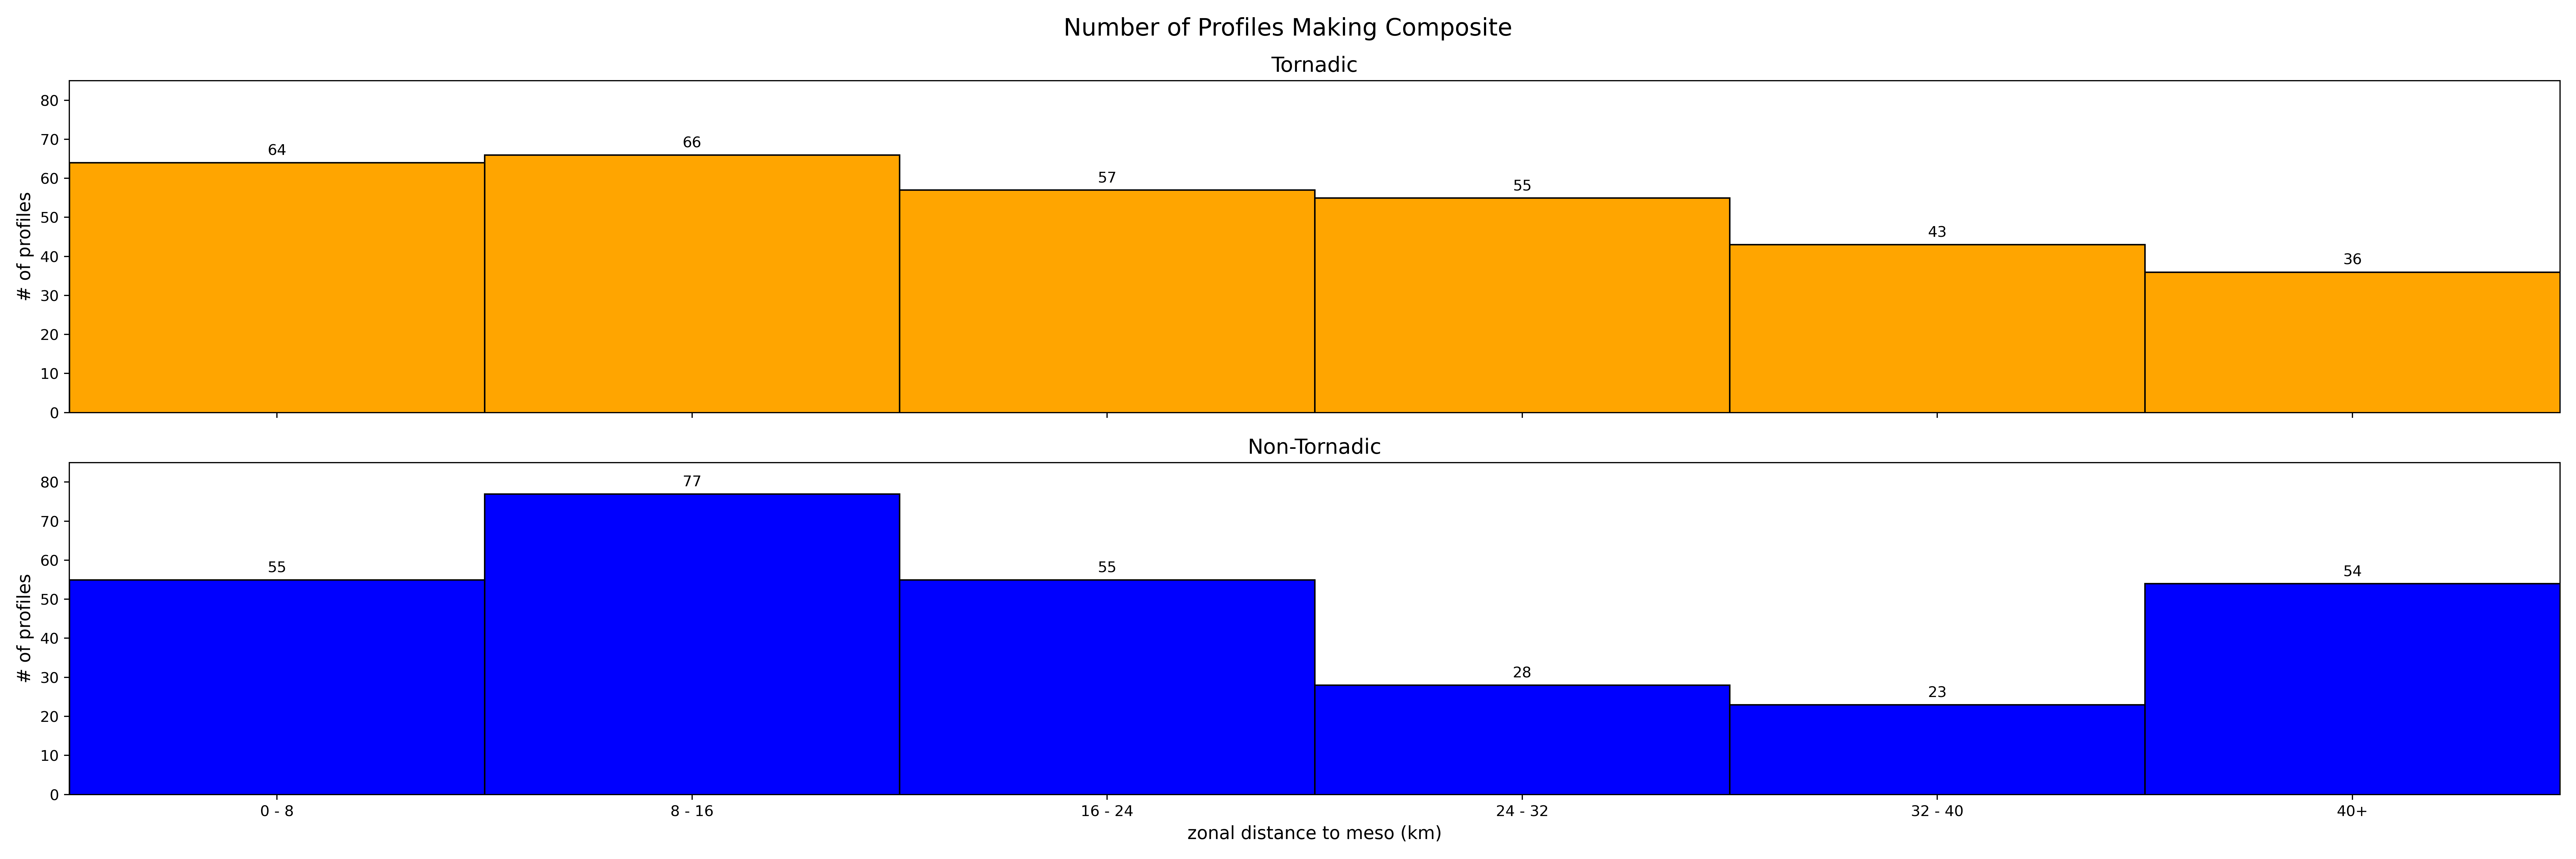
\includegraphics[width = 1\textwidth]{Figures/spatial_nprofs.png}
    \caption{Histogram of the number of WINDoe profiles making up the spatial composites used in this section. Counts for tornadic (top, orange) and non-tornadic (bottom, blue) composites are shown.}
    \label{fig:space_nprofs}
\end{figure}

\begin{figure}[h!]
    \centering
    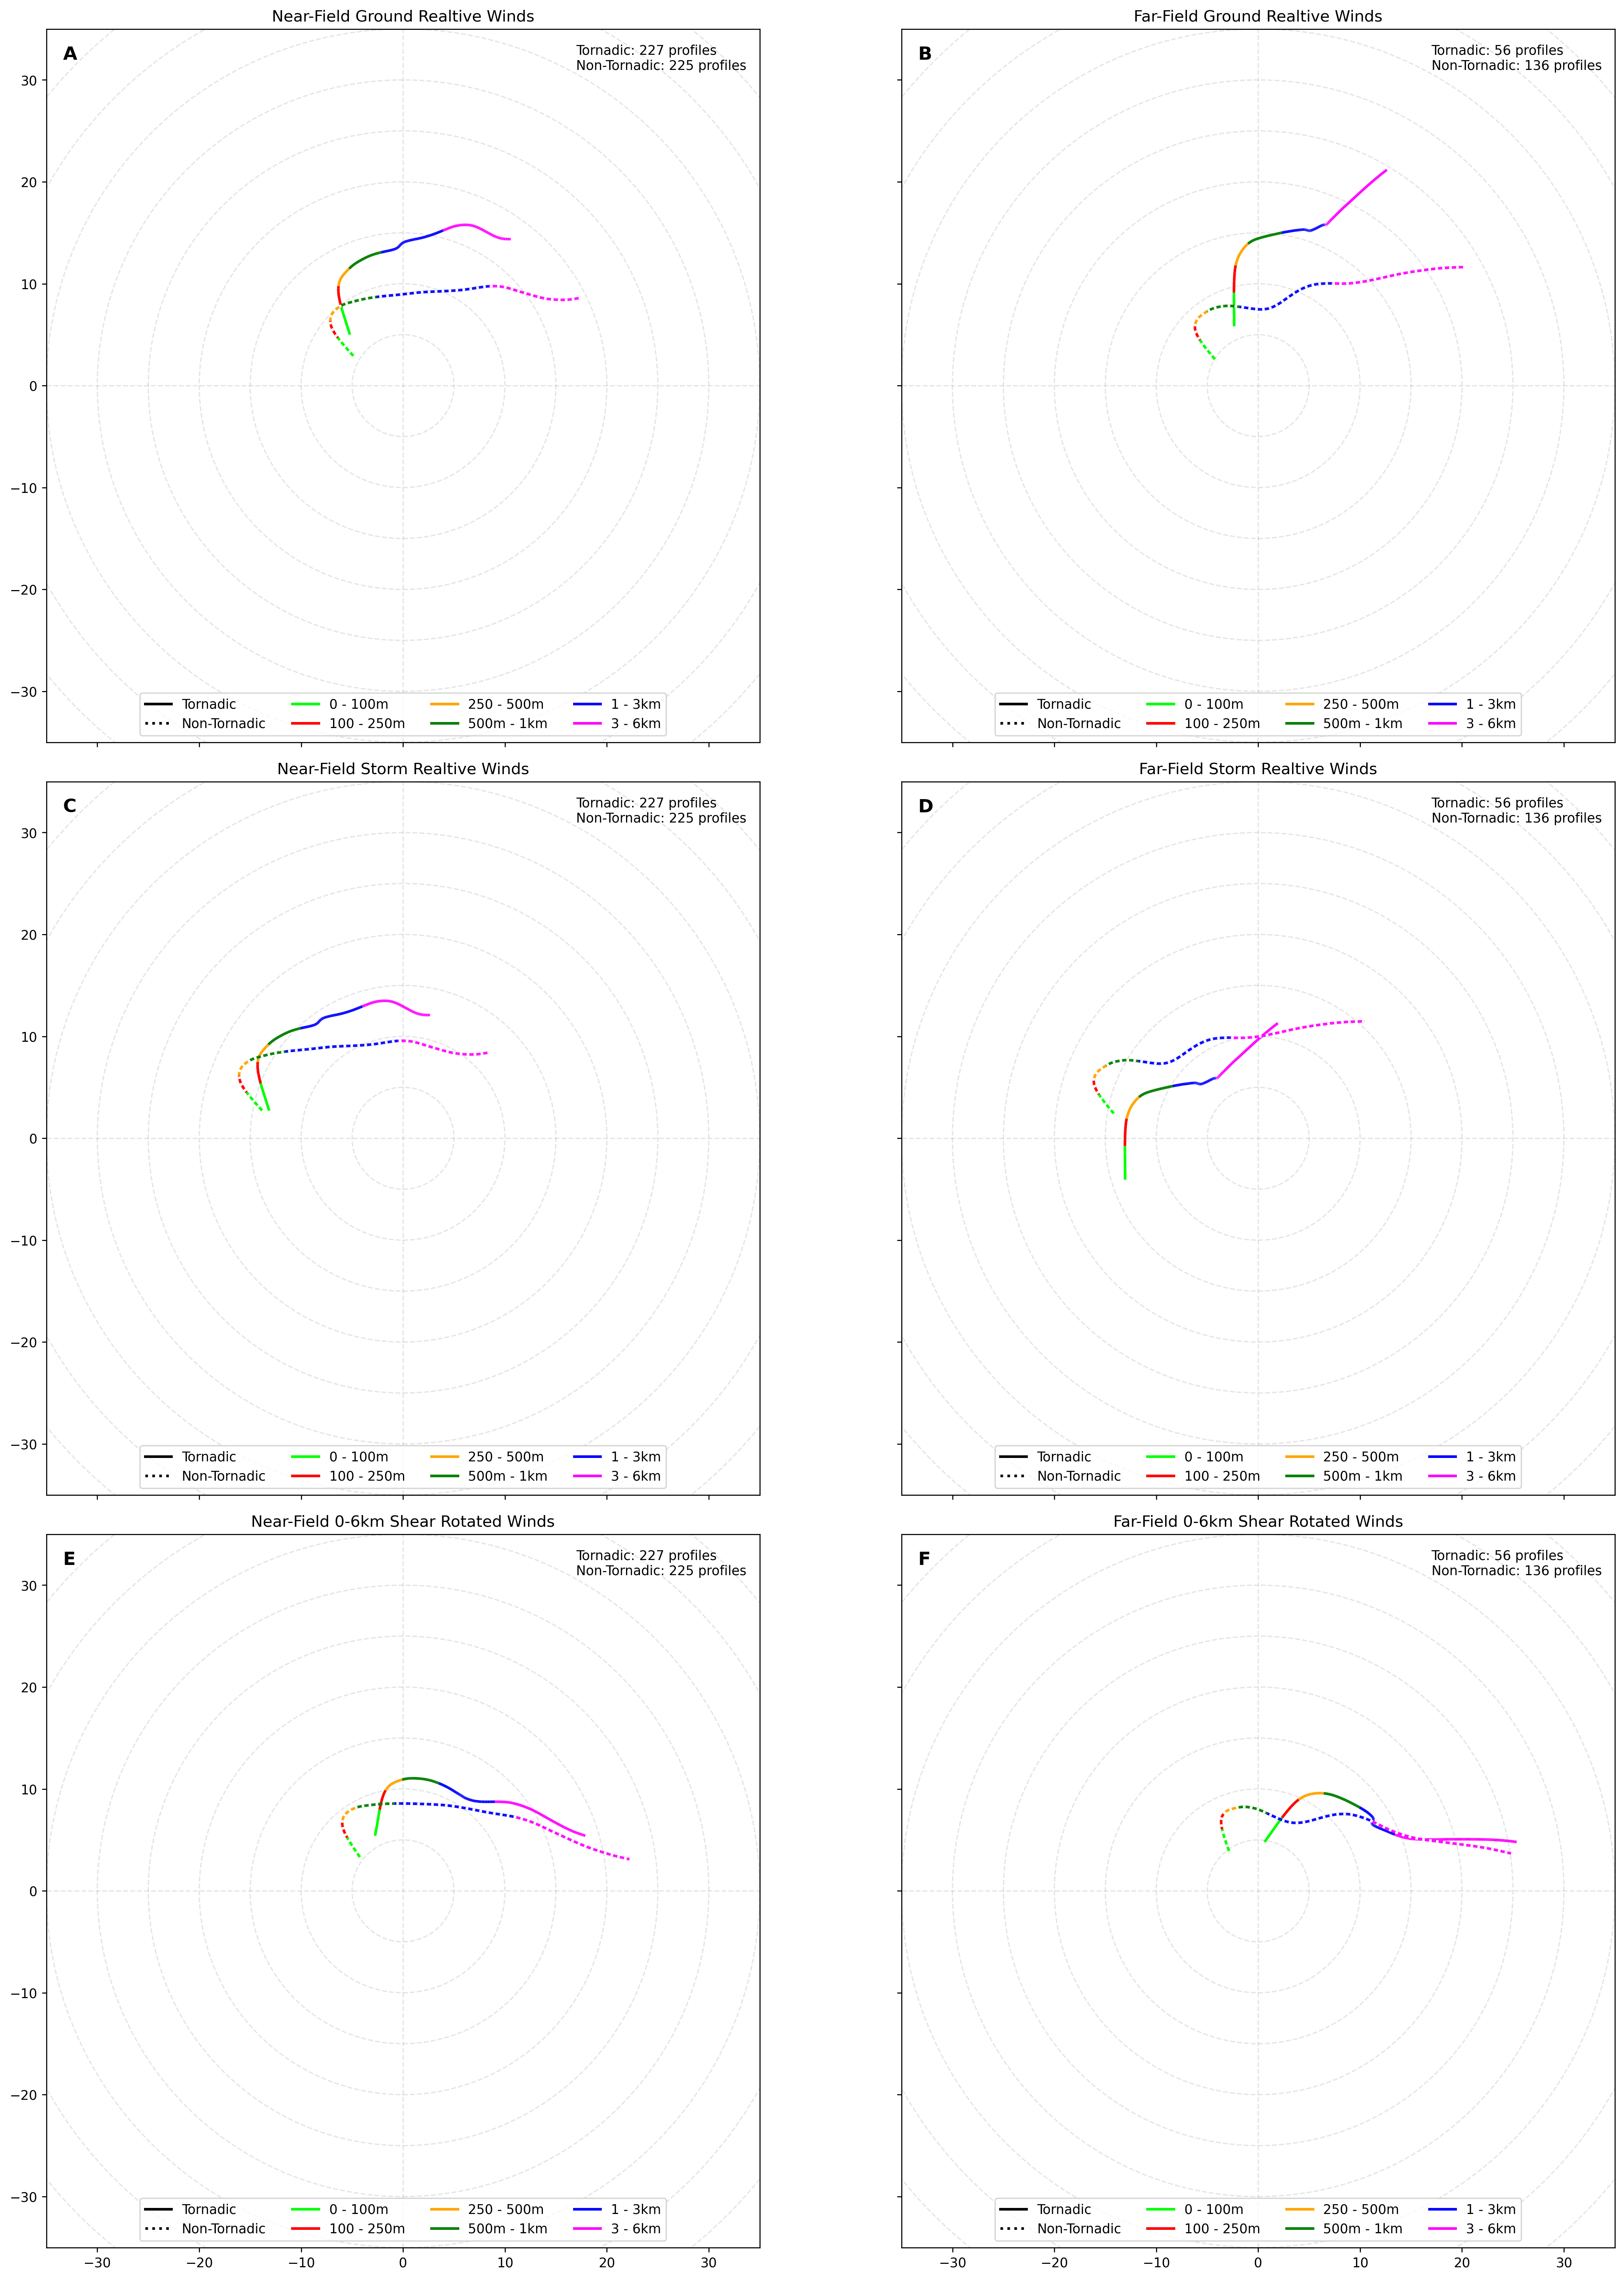
\includegraphics[width = 0.8\textwidth]{Figures/inflow_hodos_tor_no_neg.png}
    \caption{Composite ground relative (A,B; $ms^{-1}$), storm relative (C,D; $ms^{-1}$), and 0-6km shear vector rotated (E,F; $ms^{-1}$) hodographs for near-field and far-field inflow regions. Tornadic (solid) and non-tornadic (dashed) profiles are shown with the number of profiles comprising each composite shown in the respective panel.}
    \label{fig:inflow_hodos}
\end{figure}